\chapter{Modelling Methods} 
\label{Chapter4}

After all features are created, missing values handled, and outliers removed, the next step in this project is to train the various loan default models. There are four modelling techniques used in this project, namely logistic regression, random forests, extreme gradient boosting and artificial neural networks. This chapter details the datasets used to train the various models, how the features used in each model are selected, and how the parameters of each model are tuned using grid search, and how each model is validated. \\

\section{Datasets Used}

The main focus of this project is to assess if alternative data improves loan default prediction models when it is used to augment traditional credit scoring data. A secondary aim of the project is to test if accurate loan default prediction models can be developed using the alternative data features developed throughout this project. These aims are tested by training models - belonging to each of the four mentioned techniques - on all possible combinations of the 3 data categories listed in Section 3.1. The possible combinations can be seen below: 

\vspace{10pt}

\begin{itemize}
    \item sociodemographic (SD) only 
    \item credit bureau (CB) only 
    \item alternative data (ALD) only 
    \item SD and CB
    \item SD and ALD
    \item CB and ALD
    \item SD, CB and ALD
\end{itemize}

\vspace{10pt}

For each data category combination, the same dataset is used to train a model belonging to each of the 4 techniques mentioned. This means a total of 
28 models are trained. Every dataset created contains the same 60,308 loans/applicants. The number of applicants that repaid and defaulted on their loans are 47,960 and 12,714 respectively. To avoid introducing a bias towards the majority class (repaid clients) in the loan default prediction models, the classes need to be balanced before training the various models. 

\section{Class Balancing}

Imbalanced classes are a common in many classification projects. They occur when the number of observations representing one class is much lower than the number of observations representing the other classes. Imbalances pose a major issue when the "cost" of misclassifying the minority class - the class with far fewer observations - outweighs the cost of misclassifying the majority class (or classes), for example the classification of cancerous cells in the medical images \parencite{Balancing2}. \\

In the case of this project, the cost of misclassifying an applicant that is likely to default on their loan outweighs the cost of misclassifying an applicant that is likely to repay their loan. If an applicant defaults on a loan the micro-finance company granting the loan loses the loan amount lent and the potential interest that would have been gained on the loan (minus any repayments made). While, if an applicant is simply not granted a loan then the company will only lose the potential interest that would have been gained in the applicant repaid their loan.  \\

There are a variety of class balancing techniques that can be used in machine learning projects. The techniques can be broken down into two categories, algorithmic solutions and data level solutions. Algorithm solutions directly modify the the weight that each observation has on the loss function of the model being trained. While, data level solutions alter the dataset used to train models. Loss functions are used to evaluate the deviation between a model's predictions and the actual values in the data. Loss functions are minimised throughout training so that prediction error is decreased. Data level methods either involve over-sampling (copies of the minority class observations are generated) or under-sampling (only a certain percentage of the majority class observations are selected used to train the model) \parencite{Balancing1}. \\

Class balancing is completed for each of the variable combinations (datasets) detailed in Section 4.1. However, balancing is only conducted after each dataset is separated into a training and a test set, with each training set containing 80\% of the total observations and each test set containing 20\% of the total observations. Balancing is only completed after performing a train/test split so that it is possible to test for the occurrence of over-fitting due to the balancing \parencite{Balancing2}. \\

For each of the data category combinations, SMOTE - used by \textcite{NNShen} as detailed in Chapter 2 - is used to over-sample the minority class. This involves generating fictitious applicants by identifying the 5 (arbitrary selection) nearest neighbours of a randomly selected applicant that defaulted. Then calculating the variable difference vector between the applicant's features and the features of the 5 nearest neighbours. The variable difference vector is then multiplied by a random value between 0 and 1 and then added to features of the randomly selected applicant. This process is completed until the number of applicants that defaulted matches the number of applicants that repaid in each dataset. \\

After each dataset is balanced, the next step is to select the most relevant features in each dataset to be used in the modelling process. \\

\section{Feature Selection}

Feature selection is the process of determining the most relevant predictor variables for modelling purposes. \textcite{FeatureSelection} displayed that feature selection can increase the overall accuracy of a model, while decreasing the training and prediction times of a model (particularly when the training data is large). Furthermore, they found that subset and correlation coefficient selection methods outperformed other methods. \\

The following sections detail the feature selection methods used throughout this project. Initially, correlation coefficients are used to remove variables with very strong relationships to other variables. Secondly, recursive feature selection - a subset feature selection method - is used to identify the most relevant features in each of the 7 datasets used throughout this project. 

\subsection{Correlation}

Firstly, the Pearson's correlation between all independent variables is calculated. Pearson's correlations is a measure of a linear relationship between two variables \parencite{correlation1}. Figures \ref{fig:alt_cor}, \ref{fig:sd_cor}, and \ref{fig:cb_cor} display the correlation between the alternative, sociodemographic, and credit bureau variables respectively. \\

Figure \ref{fig:alt_cor} displays that there is a very strong correlation between the minimum debit and minimum balance variables. Figure \ref{fig:sd_cor} shows that there are no strong relationships between the sociodemographic variables. Figure \ref{fig:cb_cor} that there is a very strong relationship between the total number of accounts registered with credit bureaus and the total number of performing loans registered with credit bureaus. \\

\vspace{10 pt}

\begin{figure}[!htb]
\centering
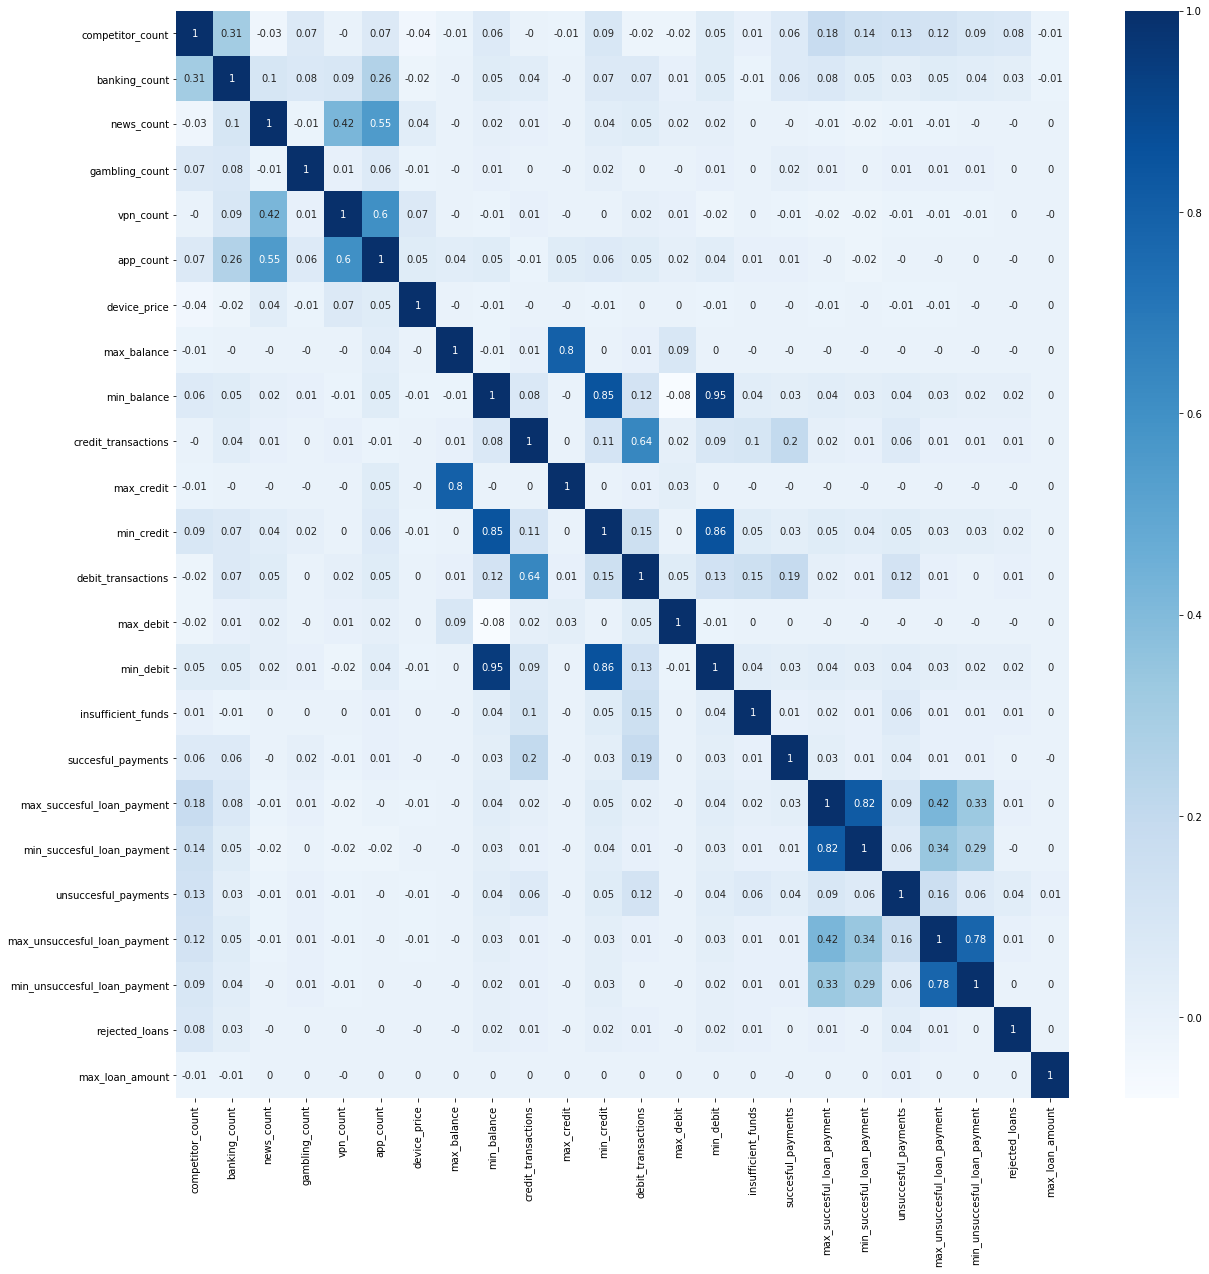
\includegraphics[width=0.55\textwidth]{images/alt_corr.png}
\caption{Correlation Between Alternative Data Variables}
\label{fig:alt_cor}
\end{figure}

\vspace{10 pt}

\begin{figure}[!htb]
\centering
  \begin{minipage}{0.5\textwidth}
    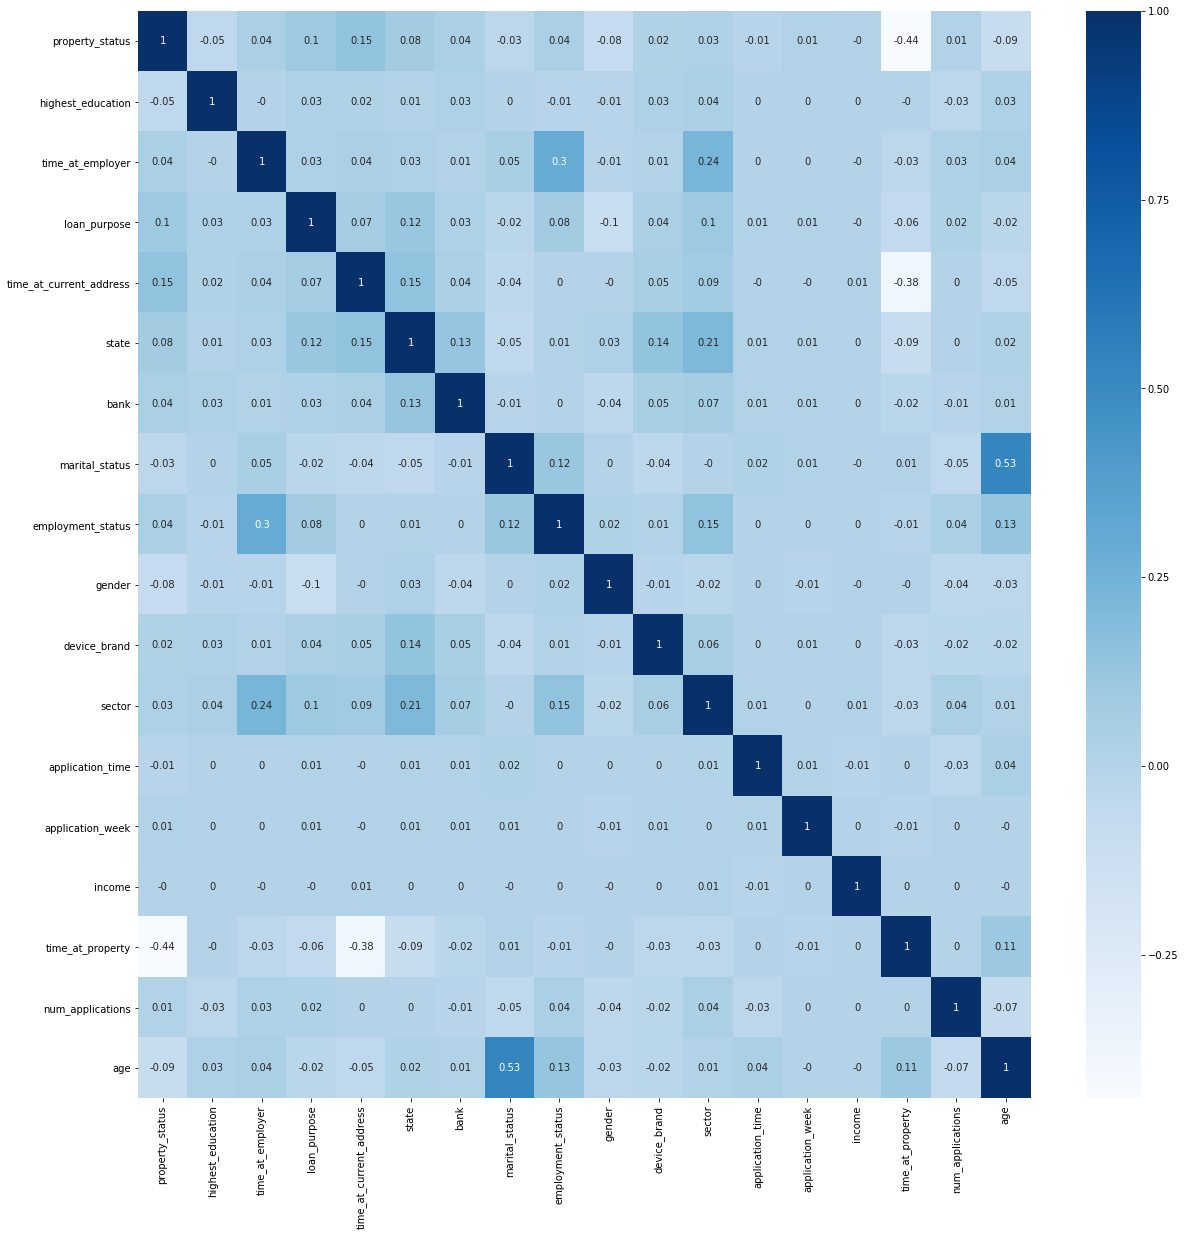
\includegraphics[width=\textwidth]{images/sd_corr.png}
    \caption{Correlation Between Sociodemographic Variables}
    \label{fig:sd_cor}
  \end{minipage}%
  \begin{minipage}{0.5\textwidth}
    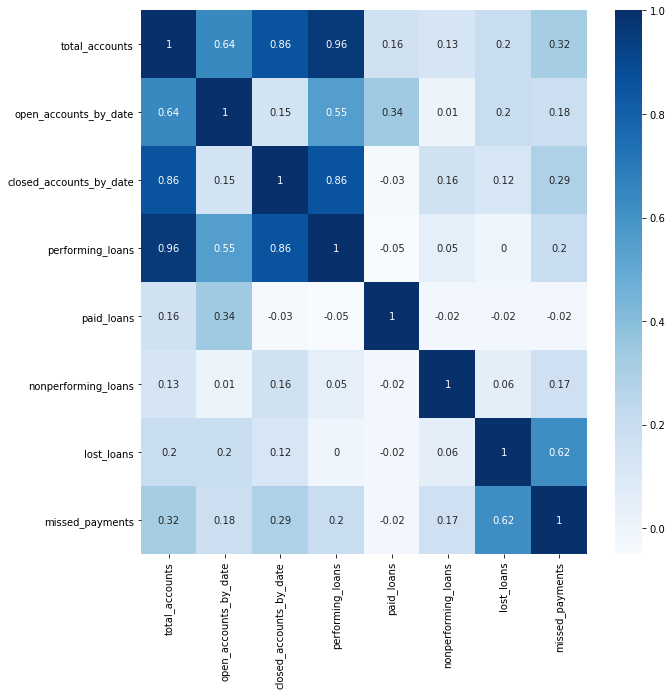
\includegraphics[width=\textwidth]{images/credit_corr.png}
    \caption{Correlation Between Credit Bureau Variables}
    \label{fig:cb_cor}
  \end{minipage}
\end{figure}

\vspace{10 pt}

To avoid capriciously selecting feature selection cut-offs based on correlation values between variables, the correlation values are only used to remove one variable from the very strong relationships (relationships over 0.9) \parencite{correlation1}. \\

Both the variations in variables that have strong relationships with other variables and the variations in variables that do not, cause variations within a model \parencite{correlation2}. Therefore, Recursive Feature Elimination (RFE) is used to select only the relevant features before each of the models are trained. 


\subsection{Recursive Feature Elimination}

Features are selected for each of the 7 datasets using RFE in conjunction with a logistic regression model. \\

RFE is an unsupervised form of subset feature selection. The technique involves recursively training a model and removing the uninformative features. For each training iteration the features used are ranked based on their importance. The weakest feature (the feature with the least importance) is removed from the training set and the model is retrained. The optimal number of features is determined by the accuracies of the models produced. This process is often validated using cross validation.  \parencite{RFE} \\

RFE reduces the dimensionality of a feature space by removing uninformative features. This decreases the training time of models, improves model performance, and eliminates dependencies and collinearity that may exist in the training data \parencite{RFE} \\

The RFE feature selection process completed in this project involves recursively retraining a logistic regression model for each feature set. The optimal number of features for each dataset is determined based upon the accuracies of the models produced and is validated using k-fold cross validation. 

\subsection{Cross Validation}

K-Fold cross validation involves partitioning the training sample of a model into k partitions. One partition serves as an independent holdout test set for the credit model being trained while the remaining k-1 partitions are used to train the model. This technique minimises the effects of data dependencies and improves the reliability of the estimates \parencite{k_fold}. Figure \ref{fig:k_fold} displays the principle of k-fold cross validation. 

\vspace{10 pt}

\begin{figure}[!htb]
\centering
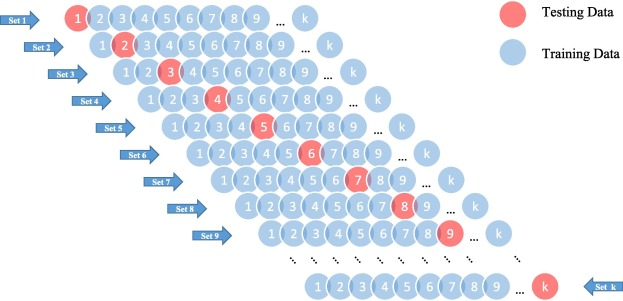
\includegraphics[width=0.75\textwidth]{images/k_fold.jpg}
\caption{K-Fold Cross Validation}
\label{fig:k_fold}
\parencite{k_fold}
\end{figure}

\vspace{10 pt}

In the case of this project, each feature selection process is validated using 5-fold cross validation. The k of the cross validation is set to 5 due to computational limitations. \\

After the most relevant features for each of the 7 datasets are selected, the optimal hyper-parameters for each models need to be determined. This is referred to as  parameter tuning. 

\section{Hyper-Parameter Tuning}

Random-search and grid-search are two of the most widely used strategies for hyper-parameter tuning in machine learning projects. Random-search is a more efficient method, but often does not lead to the most accurate models being developed \parencite{search1}. \\

Grid-search is often considered the brute force method for hyper-parameter optimisation. It involves defining possible values for each hyper-parameter of a model, then training a model for every possible combination of the defined values.  \\

Throughout this project, grid-search, in conjunction with 5-fold cross validation, is used to tune the hyper-parameters for each of the 28 models developed. 

\section{Modelling Techniques}

Once feature selection and hyper-parameter optimisation has been completed, all models are trained using only those features and parameters. A total of 7 models - one for each dataset - for each of the techniques used are trained. After training, each of the models developed are tested using a withheld 20\% validation sample (created prior to class balancing). This section details each technique used and the parameters tuned for each technique.  

\subsection{Logistic Regression}

\textcite{LogRegWiginton} first used logistic regression to develop a loan default prediction model. Since then the technique has become one of the most widely used in loan default prediction models. This is due to the techniques robustness and transparency \parencite{LogisticReg}. \\ 

As shown in Equation \ref{eq:LR}, logistic regression models - when used for loan default prediction - output the probability of an applicant defaulting of their loan. Logistic regression models are trained using maximum likelihood and the coefficients of each independent variable are estimated in such a way as to minimise the loss function. The impact of each independent variable on predictions can be directly measured through its coefficient and the importance of the variable can be determined using the variables Z score - its coefficient divided by its standard deviation.  The clarity of each coefficient and its impact is what makes logistic regression models so transparent \parencite{Hastie}. \\

The first phase in training each of the 7 models is to tune the hyper-parameters of the models using grid-search and cross validation. Each of the following hyper-parameters are tuned for each of the logistic regression models; the number of iterations completed during training, the regularisation method used, and the size of the lambda factor in the regularisation penalty (a factor which controls the magnitude of the regularisation penalty). \\

A regularisation penalty is added to the cost function of a model to shrink the size of the coefficients of the variables used. This is done to avoid over-fitting and ensure that the model generalises well \parencite{Regularisation}. In the case of the logistic regression models developed, either L1 or L2 regularisation is used. The penalty terms of L1 and L2 regularisation can be seen in \ref{eq:L1} and \ref{eq:L2} respectively. \\

\vspace{10pt}

\begin{equation} \label{eq:L1}
\lambda\sum_{j=1}^{p}|\beta_{j}|
\end{equation}

\vspace{10pt}

\begin{equation} \label{eq:L2}
\lambda\sum_{j=1}^{p}\beta_{j}^{2}
\end{equation}

\vspace{10pt}

The major difference between L1 and L2 regularisation is that L1 regularisation shrinks the coefficients of unimportant variables to zero, while L2 regularisation only shrinks the coefficients of unimportant variables towards zero \parencite{Hastie}. L2 regularisation adds the squared magnitude of a coefficient as penalty term to the loss function, while L2 regularisation adds the absolute magnitude \parencite{Hastie}. \\

After identifying the optimal hyper-parameters for each logistic regression model, each model is retained using its optimal features and hyper-parameters. The models are then tested using a withheld validation set. \\

The next technique used is random forests. The process followed to train the random forest models is discussed in the next section. 

\subsection{Random Forest}

When applied to a classification problem, the random forest algorithm involves training multiple decision trees - on independently sampled training sets ( sampled from the same overall sample) and then combining the results of the various classifications of the trees using a voting process \parencite{RandomForest}. \\

Each tree in the forest is grown while meeting the following conditions:

\begin{itemize}
    \item If there are N observations in the overall training sample, a training set is created by sampling N observations - with replacement - from the overall sample. 
    \item If there are M dependent predictor variables in the overall training set, the sample training set consists of m (where m<=M) randomly sampled predictor variables. 
    \item Each tree trained is grown to its largest possible extent (no pruning is completed) \parencite{RandomForest}.
\end{itemize}

\textcite{BagWang} and \textcite{BigDataMicroFiance} have shown that the random forest algorithm can successfully be applied to loan default prediction. In the case of this project a random forest model is trained for each of the 7 data category combinations. Each model is tested using an unseen validation set. During training the hyper-parameters of each model are tuned using a grid-search. 

\subsubsection{Parameter Tuning}

Each random forest model has the following hyper-parameters tuned during training:

\begin{itemize}
    \item The number of trees grown in the forest.
    \item The maximum number of features used within a particular forest. 
    \item The maximum depth (the maximum number of splits) of each tree in the forest.
    \item The minimum number of observations required within each node for a split to be allowed. 
\end{itemize}

Tuning the above hyper-parameters of each random forest model allows for the most accurate and generalizable models to be developed. The process ensures that the trees contained within each random forest model are diverse, thus reducing the likelihood of over-fitting to the training data \parencite{RF_Tuning}. \\

The criterion used to measure the quality of splits within each tree is Gini impurity, this is the same measure used by \textcite{DecTreesZekic}. Another criterion option is Shannon Entropy, however this is more computationally intensive than Gini impurity \parencite{Gini}. \\

After the each random forest model's optimal hyper-parameters have been identified and validated, the models are retrained using only those parameters. The models are then tested using a holdout validation set. \\

The next machine learning technique used is Extreme Gradient Boosting (XGBoost), this technique will be discussed in the following section. 

\subsection{Extreme Gradient Boosting}

Gradient boosting is a machine learning technique that involves developing a model which is an ensemble of weak prediction models. Typically, the models in the ensemble are decision trees. A gradient boosted model is trained in a stage-wise fashion, the model is generalised by minimising a defined loss function throughout training \parencite{Boosting}.   \\

The final output of a tree ensemble model is calculated by summing the predictions of each tree in the ensemble, varying weights can be attached to the predictions of specific trees This technique is shown in Figure \ref{fig:tree_ens}. \\

\vspace{10 pt}

\begin{figure}[!htb]
\centering
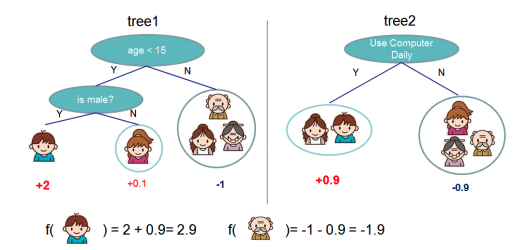
\includegraphics[width=0.75\textwidth]{images/tree_ensemble.png}
\caption{Example of a Tree Ensemble}
\label{fig:tree_ens}
\parencite{XGBoost}
\end{figure}

\vspace{10 pt}

The XGBoost technique was developed by \textcite{XGBoost}. Its derivation spawned from second order method developed by \textcite{Boosting}. \textcite{XGBoost} altered the regularised learning objective developed by \textcite{Boosting} to improve the performance of XGBoost models. They proposed that for any given dataset, with n observations and m predictor variables, a tree ensemble model can be represented by using K additive functions  shown in Equation \ref{eq:xgb_reg}. 

\vspace{10pt}

\begin{equation} \label{eq:xgb_reg}
\hat{y}_{i} = \sum_{k=1}^{k}f_{k}(x_{i}), f_{k} \varepsilon F,
\end{equation}

\vspace{10pt}


Where $\hat{y}_{i}$ is a predicted valued and $F = {f(x) = w_{q(x)}}(q : R^{m}$ → $T, w \varepsilon R^{T})$ is the space of ensemble decision trees. While q represents the structure of each tree and T is the number of leaves (terminal nodes) in the tree. Each $f_k$ corresponds to an independent leaf (q) and leaf weights (w). The weight on the i-th leaf is represented by $w_i$ \parencite{XGBoost}. \\

In gradient tree boosting, the set of regularised functions that represent the ensemble of trees are learnt in an additive manner by minimising the loss functions associated to each predicted value. A general version of a loss function used in XGBoost is shown in Equation \ref{eq:xgb_loss}. Loss functions measure the difference between the predicted target values shown in Equation \ref{eq:xgb_reg} and the known target values. 

\vspace{10pt}

\begin{equation} \label{eq:xgb_loss}
\tilde{L}^{k} = \sum_{i=1}^{n}l(y_i,\hat{y}_{i}^{k-1} + f_k(x_i))+ \Omega(f_k)
\end{equation}

\vspace{10pt}

The $f_k$ that best improves the model is greedily added when a loss function is minimised. Second-order approximation is used to simplify the optimisation of each loss function. The simplified version can be seen in Equation \ref{eq:xgb_second}.

\vspace{10pt}

\begin{equation} \label{eq:xgb_second}
\tilde{L}^{k} = \sum_{i=1}^{n}[g_i f_k(x_i) + \dfrac{1}{2} h_i f^{2}_{k}(x_i)] + \Omega(f_k)
\end{equation}

\vspace{10pt}

Where $g_i$ and $h_i$ are first and second order gradient statistics on the loss function. If we define an instance of leaf j as $I_j = {i|q(x_i) = j}$ then we can expand the $\Omega$ in Equation \label{eq:xgb_second} so that the Equation now appears as below in Equation \ref{eq:xgb_expanded}. 

\begin{equation} \label{eq:xgb_expanded}
\tilde{L}^{k} = \sum_{i=1}^{n}[g_i f_k(x_i) + \dfrac{1}{2} h_i f^{2}_{k}(x_i)] + \lambda T + \dfrac{1}{2} \lambda \sum_{j=1}^{T} w^{2}_{j}
\end{equation}

\vspace{10pt}

We can then compute the optimal weight and corresponding value of a fixed structure as shown in Equations \ref{eq:xgb_weight} and \ref{eq:xgb_value}. 

\vspace{10pt}

\begin{equation} \label{eq:xgb_weight}
w^{*}_{j} = - \dfrac{\sum_{i \varepsilon I_{j}} g_i}{\sum_{i \varepsilon I_{j}} h_i + \lambda}
\end{equation}

\vspace{10pt}

\begin{equation} \label{eq:xgb_value}
\tilde{L}^{k}(q) = - \dfrac{1}{2} \sum_{j=1}^{T} \dfrac{\sum_{i \varepsilon I_{j}} g_i}{\sum_{i \varepsilon I_{j}} h_i + \lambda} + \lambda T
\end{equation}

\vspace{10pt}

Figure \ref{fig:xgb_score} displays how the optimal values are calculated for each terminal node of a tree. This is done in a greedy manner. The algorithm starts with a single node and iteratively adds branches \parencite{XGBoost}.\\

Beyond the regularised learning of loss function, the XGBoost algorithm uses two techniques to avoid over-fitting. These techniques are shrinkage and feature sub-sampling (this technique is used in random forests). Shrinkage scales the weights of trees by weights by a of $\eta$. This reduces the impact a single tree has on the final output of a model \parencite{Shrinkage}. \newpage

\vspace{10 pt}

\begin{figure}[!htb]
\centering
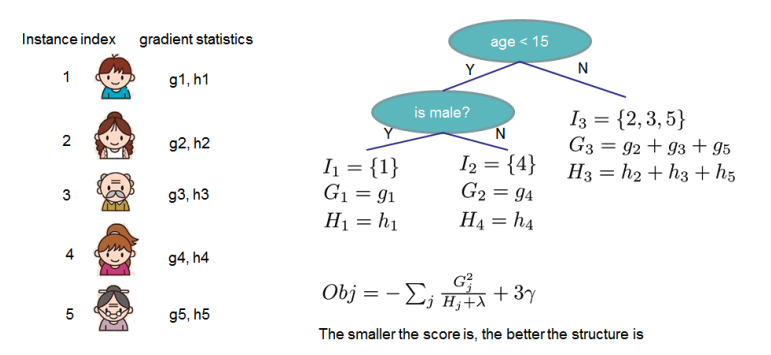
\includegraphics[width=0.75\textwidth]{images/tree_score.png}
\caption{How Leaves are Scored in XGB}
\label{fig:xgb_score}
\parencite{XGBoost}
\end{figure}

\vspace{10 pt}


\textcite{Ensemble} displayed that the XGBoost technique can effectively be applied to credit scoring.Their XGBoost model outperformed the logistic regression, random forest, and neural network models they developed for comparative purposes in overall prediction accuracy, area under the curve, and Brier score. \\


\textcite{Ensemble} used Bayesian optimisation to tune the hyper-parameters of their XGBoost model. In the case of this project grid-search is used to train the hyper-parameters of the XGBoost models developed. The following subsection details the parameters tuned. 

\subsubsection{Parameter Tuning}

The hyper-parameters tuned for each XGBoost model are as follows:

\begin{itemize}
    \item Eta, which is the factor by which new weights are shrunk. This prevents over-fitting.  
    \item Gamma, which is the minimum loss required before a split should be made in a tree. A large Gamma value will result in fewer splits and as a result a more conservative model. 
    \item Maximum depth, the maximum number of splits in a tree. 
    \item Minimum child weight, the minimum sum of weights required in a tree. The larger the minimum child weight the more conservative the model. 
    \item Sub-sample, which is the ratio of the training data that is sub-sampled when a tree is grown. 
    \item Column sample by tree, is the ratio of predictor variables used in each tree. 
\end{itemize}

Similarly to hyper-parameter tuning in random forest model, parameter tuning in XGBoost models have a two fold purpose. It aids in the most accurate models being developed but it also prevents over-fitting from occurring \parencite{xgb_tuning}. Furthermore, the learning objective of the XGBoost models is set to be a binary classification and the evaluation metric is set area under the curve. The later is done so that the XGB models generalise well. \\

After hyper-parameter tuning the models are retained using the most optimal parameters and are then tested using a holdout set. After the XGBoost models are trained and tested, the same process is completed for the 7 neural network models developed.  


\subsection{Neural Networks}

Artificial neural networks (NN's) consist of a network of interconnected processors termed neurons. Each neuron receives an input and processes it by passing it through its activation function. Input neurons receive raw input, while other neurons in the network receive a weighted input from previously activated neurons. The learning aspect of a neural network involves adjusting the weights of connections so that the network outputs more desirable results. This process is carried out by back propagation and often involves minimising a loss function so that the predicted values produced by a network are as close as possible to the true values of data points used to train the network \parencite{NNOverview}. \\ 

Neural networks have a variety of architectural structures. Recently recurrent neural network (RNN) architectures (networks that contain contain cyclic connections between neurons) such as long short-term memory networks have become prominent. These networks are well suited to modelling temporal or sequence behaviour \parencite{LSTM}. \\

\textcite{DecTreesZekic} have shown that neural networks can be successfully applied to loan default prediction. While, \textcite{NNWest} explored the various architectures, activation functions, and loss functions that can be used when training a NN used for loan default prediction. \\

In the case of the loan default prediction NNs developed throughout this project, no temporal or sequential behaviour is modelled and therefore an RNN architecture is not required. \textcite{NNWest} displayed that multi-layer perceptrons (MLPs) are effective models when used for loan default prediction. MLPs are an example of feed-forward neural networks, which means that their neurons are connected in a one-directional fashion \parencite{NNOverview}. An example of a three layer MLP can be seen in Figure \ref{fig:MLP}.

\vspace{10 pt}

\begin{figure}[!htb]
\centering
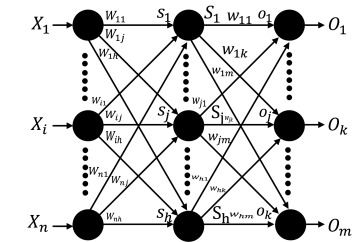
\includegraphics[width=0.85\textwidth]{images/mlp.jpg}
\caption{Architecture of a Multi-Layer Perceptron}
\label{fig:MLP}
\parencite{MLP}
\end{figure}

\vspace{10 pt}

The neurons on the left of the Figure represent the input layer, the central neurons form the hidden layer, while the neurons on the right represent the output layer. MLPs can have numerous hidden layers but always have only one input and output layer. The number of neurons in the input layer always matches the number of variables used in the model.  \parencite{MLP}. \\

Each neuron in a neural network has an activation function. Activation functions map the weighted input a neuron receives to the output signal the same neuron produces. Activation functions can be linear or non-linear. They are often used to limit or smooth the output of a particular neuron. Activation functions commonly used in MLPs are sigmoid, hyperbolic tangent, radial bias, rectified linear unit (ReLU), and softmax \parencite{activation_functions}. \\


Predictions in an MLP model are calculated using Equation \ref{eq:MLP}

\vspace{10pt}

\begin{equation} \label{eq:MLP}
y_m = \sum_(i=1)^{n}(W_{ij} X{i}) - \theta_j     j = 1,2,...,h
\end{equation}

\vspace{10pt}

Where $W_{ij}$ represents the weight connecting the i-th neuron to j-th-neuron, $\theta_j$ represents the bias of the j-th-neuron, and $X_i$ represents the input data to the i-th neuron \parencite{MLP}. \\

In the case of the NNs developed throughout this project, the input layer of each NN developed contains the same number of neurons as the number optimal features identified during feature selection. While the output layer contains a single neuron with a sigmoid activation function. If the weight inputted into the final neuron is below a certain value then the applicant is deemed to be likely to default. The optimal cut-off value is learnt through back propagation. \\ 

NNs, like the aforementioned models, have many hyper-parameters that need to be optimised. Again, this process is completed using a combination of grid-search and cross-validation. In the case of the NNs, the optimisation serves a two fold purpose. The first is to identify the parameters which result in the most accurate and generalizable model, while the second is to find the architecture which leads to the most accurate model and generalizable model. In the case of this project, the optimal number of hidden layers and  the optimal number of neurons in each hidden layer is determined using grid-search and cross-validation. 

\subsubsection{Parameter Tuning}

The hyper-parameters tuned for each NN model are as follows:

\begin{itemize}
    \item Learning rate, which determines how quickly a network updates its parameters. The smaller the learning the slower a model trains. A larger learning rate results in a model training faster but can result in weights not converging \parencite{NN_HP}. This principle is displayed in Figure \ref{fig:learning_rates}. 
    
    \vspace{10 pt}

    \begin{figure}[!htb]
    \centering
    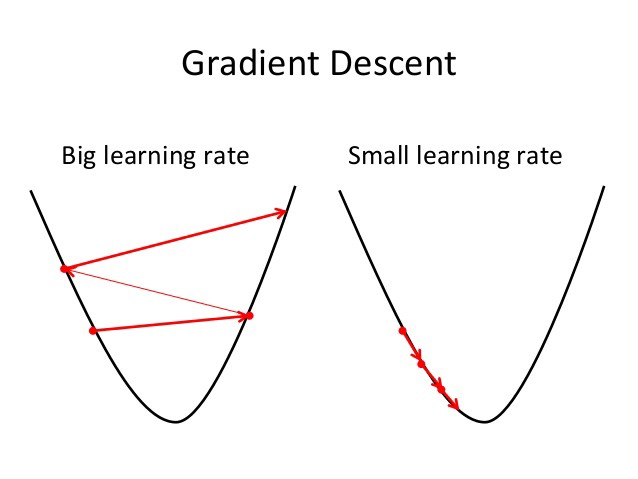
\includegraphics[width=0.32\textwidth]{images/learning_rate.jpg}
    \caption{Varying Learning Rates}
    \label{fig:learning_rates}
    \parencite{learning_rate}
    \end{figure}
    
    \vspace{10 pt}
    
    \item Dropout rate, which is the percentage of neurons that are randomly removed from the network during training. Dropout aims to prevent over-fitting and increase a model's generalizing power \parencite{learning_rate}. 
    
    \item The number of training iterations. The number of forward and back passes used to train the network \parencite{NN_HP}.
    
    \item The batch size, which is the number of training observations used in a forward/back training pass \parencite{NN_HP}. 
    
    \item The architecture of the network: the number of hidden layers in the network and the number of neurons in each hidden layer. 

\end{itemize}

 
\vspace{10 pt}

Hyper-parameters that were set but not optimised were the loss function and the activation functions of the output neuron. A sigmoid cross-entropy loss function is used in the MLP models. This is not an arbitrary selection, the Python package used to developed the MLP models only supports this loss function for binary classification problems. As previously stated the activation function of the output neuron is set to a sigmoid function. \\

After the hyper-parameters of each NN model are identified, each model is tested using a holdout set.
